\textbf{\Large Resultate}
\vspace*{1.6em}\\
Bei den Testmessungen traten keinerlei Gerätefehler oder Störungen auf, sodass für alle 28 Probanden Ergebnisse in Form von Graphen erstellt werden konnten. Abb. 2 zeigt ein Beispiel einer 6-Felder-Grafik, in der die angewandten Methoden in mehreren Feldern aufgetragen sind. Zum Ablesen der ventilatorischen Schwellen ist die entsprechend gemessene Herzfrequenz in Form einer rosafarbenen Linie in die Plots integriert. Einige der Graphen waren jedoch nicht-differenzierbar und daher nur erschwert optisch auszuwerten.

\begin{center}
\begin{picture}(\spaltenbreite,16)
\put(-2.5,3){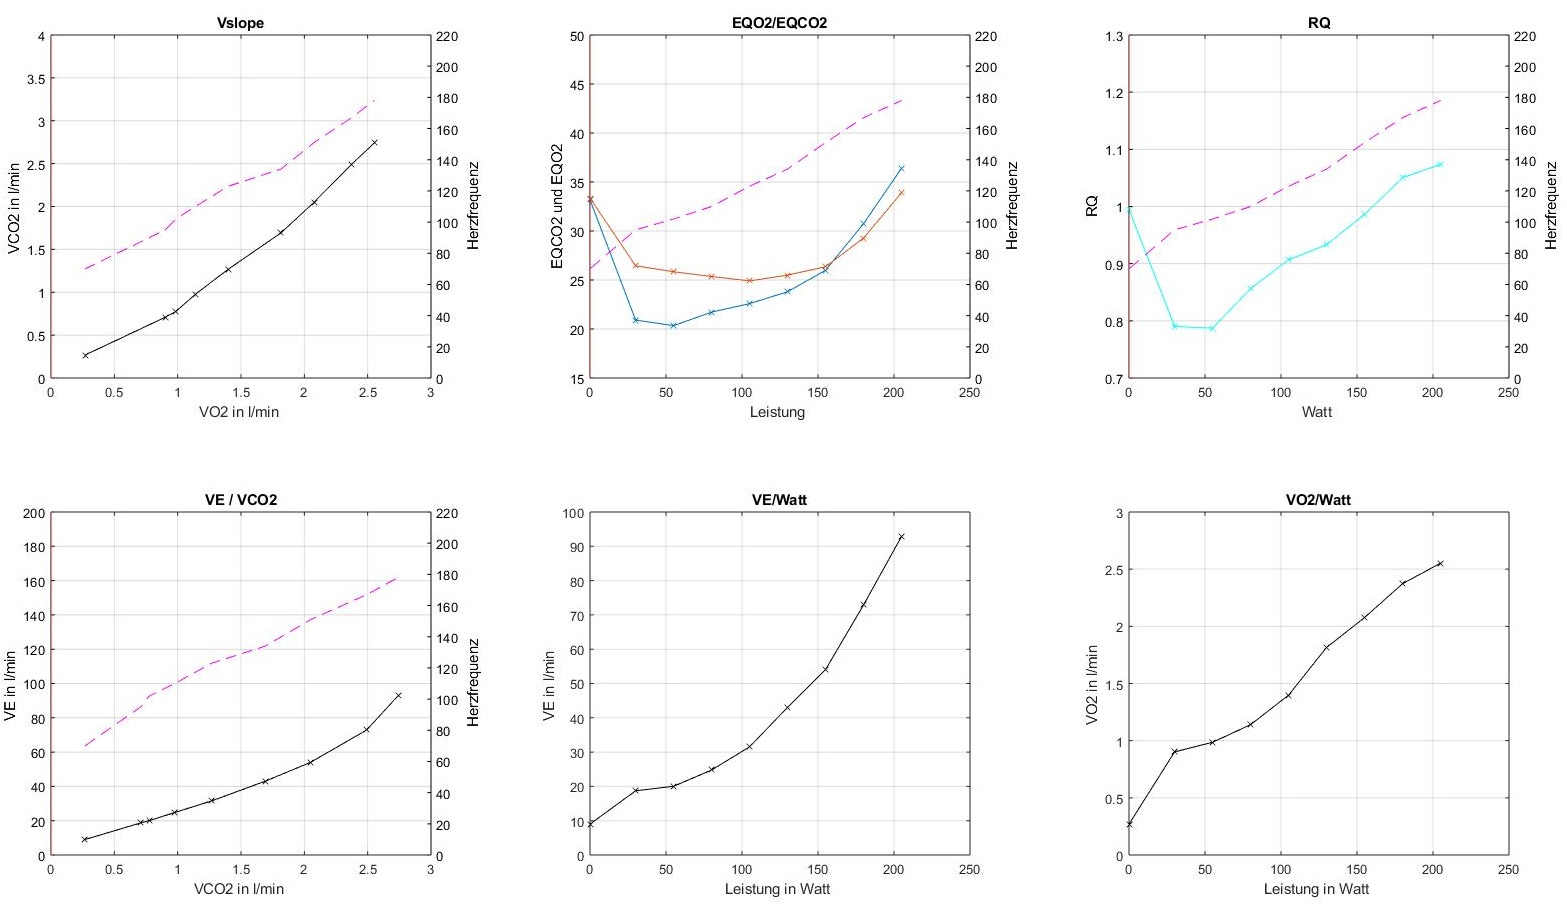
\includegraphics[width=200mm]{Bilder/plot_6w.jpg}}
\put(1.3,1.5){\parbox{720pt}{{\bf \small Abb. 2:} \small Beispiel einer 6-Felder-Grafik}}
\end{picture}
\end{center}

